%%%%%%%%%%%%%%%%%%%%%%%%%%%%%%%%%%%%%%%%%
% fphw Assignment
% LaTeX Template
% Version 1.0 (27/04/2019)
%
% This template originates from:
% https://www.LaTeXTemplates.com
%
% Authors:
% Class by Felipe Portales-Oliva (f.portales.oliva@gmail.com) with template 
% content and modifications by Vel (vel@LaTeXTemplates.com)
%
% Template (this file) License:
% CC BY-NC-SA 3.0 (http://creativecommons.org/licenses/by-nc-sa/3.0/)
%
%%%%%%%%%%%%%%%%%%%%%%%%%%%%%%%%%%%%%%%%%

%----------------------------------------------------------------------------------------
%	PACKAGES AND OTHER DOCUMENT CONFIGURATIONS
%----------------------------------------------------------------------------------------

\documentclass[
	12pt, % Default font size, values between 10pt-12pt are allowed
	%letterpaper, % Uncomment for US letter paper size
	%spanish, % Uncomment for Spanish
]{fphw}

% Template-specific packages
\usepackage[utf8]{inputenc} % Required for inputting international characters
\usepackage[T1]{fontenc} % Output font encoding for international characters
\usepackage{mathpazo} % Use the Palatino font

\usepackage{graphicx} % Required for including images

\usepackage{booktabs} % Required for better horizontal rules in tables

\usepackage{listings} % Required for insertion of code

\usepackage{enumerate} % To modify the enumerate environment

\usepackage{caption}

\usepackage{listings}

\usepackage{float}

\usepackage{relsize}
\usepackage{xcolor}
\usepackage{verbatim}

\definecolor{mygreen}{rgb}{0,0.6,0}
\definecolor{mygray}{rgb}{0.5,0.5,0.5}

\lstset{language=Python,%
	%basicstyle=\color{red},
	breaklines=true,%
	keywordstyle=\color{blue},
	morekeywords=[2]{1}, keywordstyle=[2]{\color{black}},
	identifierstyle=\color{black},
	stringstyle=\color{gray},
	commentstyle=\color{mygreen},
	numberstyle=\tiny\color{mygray}, % the style that is used for the line-numbers
           rulecolor=\color{black},
	showstringspaces=false,
	emph=[1]{for,end,break},emphstyle=[1]\color{green},
	}

%----------------------------------------------------------------------------------------
%	ASSIGNMENT INFORMATION
%----------------------------------------------------------------------------------------

\title{Deep Learning on Kubeflow} % Assignment title

\author{ Iurii Mozzhurin \& Rebekka Pech} % Student name

\date{July 28th, 2019} % Due date

\institute{Goethe University Frankfurt am Main}% \\ Big Data Lab} % Institute or school name

\class{Hands-on Lab - Big Data Technologies SS 2019} % Course or class name

%----------------------------------------------------------------------------------------

\begin{document}

\maketitle % Output the assignment title, created automatically using the information in the custom commands above

%----------------------------------------------------------------------------------------
%	ASSIGNMENT CONTENT
%----------------------------------------------------------------------------------------

\vspace{80pt}

\section{Introduction to Kubeflow}

Kubeflow is an open-source platform that is based on Kubernetes and was developed by Google. It's dedicated for making deployments of Machine Learning workflows on Kubernetes simple, portable (it works on any Kubernetes cluster) and scalable (upon need). Kubeflow makes it possible to bring ML in any existing cluster \cite{kf}. \\

When talking about Kubeflow (KF) you also have to talk about Kubernetes. Kubernetes is an open-source container-orchestration system. With Kubernetes you only need to define what resources the app needs, how many instances should be made, and Kubernetes takes care of deploying, managing and balancing containers on the hardware (nodes).\\  

The main idea of Kubeflow is that it's a ready-to-use set of Machine Learning tools. It's not necessary to install and connect the tools separately, but it can be done automatically. It also provides GUI, which makes the work with them easy for non-programmers.\\

Kubeflow includes components for model developing, training and serving and also for hyperparameter tuning and pipelines.\\

Kubeflow should be used for distributed ML workflow, for ML in production or for ML in the cloud.
\ \\
%%%%%%%%%%%%%%%%%%%%%%%%%%%%%%%%%%%%%%%%%%%%%%%%%%
\pagebreak
\section{Use Case Setup}

The intention of our use case was to train a convolution neural network to distinguish between works of ten
painters. In the end, we wanted to have a (good) prediction when we give an image into our model whose painting it is.\\

For this model, we used the Dataset ``Painter by Numbers'' from kaggle.com \cite{kaggle} which has an original size of 83GB  but that includes a lot of images from many more than 10 artists. Most of the images were from WikiArt.org. In the original dataset we had image dimensions from 477 to 7444 Pixels.\\

\begin{figure}[H]
	\center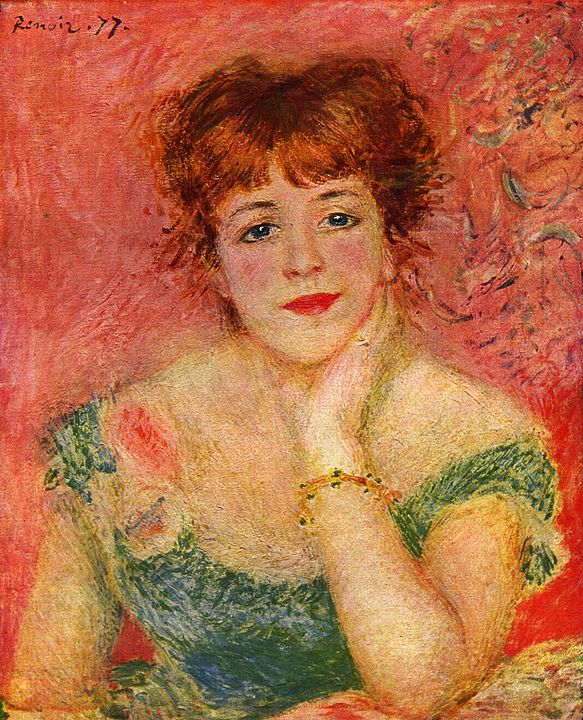
\includegraphics[width=0.2 \textwidth]{Renoir.jpg}
	\caption{Example painting of \textit{P.Renoir}}
\end{figure}

We selected a small part of this data and also resized it to 448 Pixels on the smallest side. Therefore, in the end, we worked with 340 MB. By that, we had 388 images per artist from 10 different painters. From these images we used 20 images per artist only for the validation - that's 5 percent of all data - and the rest was used for the training of the model.\\

\subsection*{ResNet-50}
\ \\  

We have decided to use transfer learning, the technique often applied for small datasets, where a model is first trained on a much larger dataset, which is different from the main dataset. In this case, the model learns some important features of images, those later can be utilized to classify our target images.  

For the use case, we selected \textit{ResNet-50} model \cite{resnet}, which is known for good results in image recognition, trained on more than a million images from the \textit{ImageNet} database. This residual convolution network is 50 layers deep and can classify images into 1000 object categories. To adapt the model for our task, we swapped the last layer of 1000 units with a layer of 10 units, fixed the weights in the rest of the network and during transfer learning trained only the last layer.  \\

Later on, we have also modified our code, so it can be used to train the whole model, and tried the full training from scratch along with transfer learning.

\begin{figure}[H]
	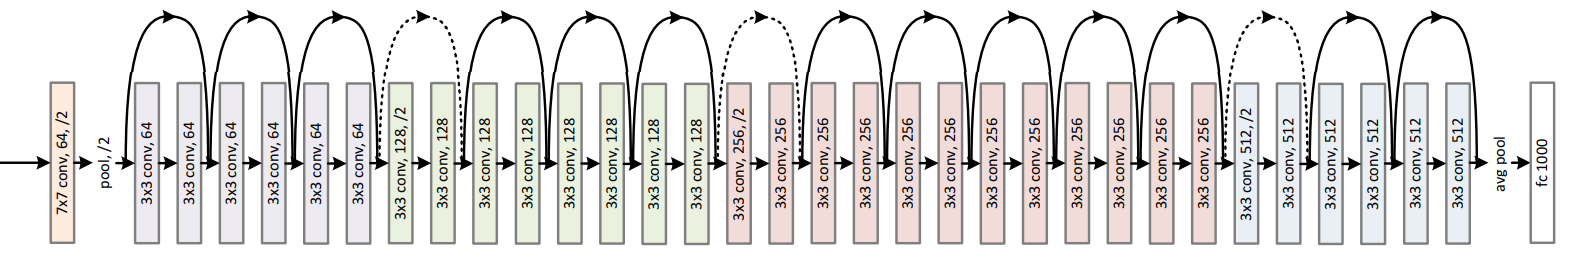
\includegraphics[width=1\textwidth]{resnet.png}
	\caption{Scheme of ResNet-34 from \cite{resnet}. Our model ResNet-50 has the same architecture but 50 layers instead of 34.}
\end{figure}

During training, we used different random image transformations, such as shift, rotation, and flip. This method is called image augmentation and used to prevent overfitting, so the model cannot just memorize all training images but is forced to learn some generalizations from them.\\

\subsection*{Milestones}
\ \\  

When we started our use case, we made a plan of the milestones we want to achieve. These are the objectives we had at the beginning:
\begin{enumerate}
\item Install the software and deploy Kubeflow on GCP 
\item Preprocess the data
\item Create a model for transfer learning in Python
\item Create a Docker image for this model
\item Train the model on GKE using TFJobs on CPUs
\item Save the trained model
\item Train the model on GKE using TFJobs on GPUs
\item Perform distributed training on multiple pods
\item Serve the model with TF Serving
\end{enumerate}


\subsection*{Technologies}
\ \\ 

To exploit most of Kubeflow's functionality, we decided to deploy it on Google Cloud Platform (GCP), so we could try training on high-performance machines, with graphic accelerators and distributed training. To manage the deployment we used the GCP console, \verb|gcould| and \verb|gsutil|.\\

We wanted to implement the model in Tensorflow(TF) because KF was originally developed by Google specifically for this framework, but soon have switched to Keras (with TF as a back-end). First, because TF is a pretty complicated package and requires additional time to study it. And second, transfer learning in TF is officially implemented using Keras \cite{tf}.\\

Keras is a front-end for different machine learning frameworks \cite{keras}, previously as a stand-alone library but now it is adopted as part of several packages including TF. It simplifies the usage of neural networks but lacks functionality.\\

For the containers, we used Docker and Kubernetes as the main technologies in this field and also parts of KF. \\

There are several ways to train a model in KF and we decided to use TFJobs on separate pods for this project. To manage the pods we previously wanted to use \verb|kubectl| and \verb|ksonnet|. The second one is used to create a template for a Kubernetes pod, and the first - to deploy the pod from the template. Unfortunately, \verb|ksonnet| was depreciated and removed from KF during our work on the project. It was replaced by \verb|kustomize| but large parts of the documentation and tutorials still were not updated. After unsuccessfully spending lots of time on \verb|kustomize|, we have developed the template for the training node by hand and applied it with \verb|kubectl|.\\

Pods in Kubernetes are temporal, after finishing their task (like training) they will be deleted. So for storing the dataset, the trained model and the logs we needed persistent storage. First, we planed to use for these porpoises a Persistent Volume Claim (PVC), a special pod with storage space, but its management in KF requires \verb|ksonnet|, so for storing the model we decided to use a bucket on Google Cloud Storage (GCS) and the dataset was stored on a public host on the Internet (Dropbox).\\

For the monitoring we wanted to use Tensorboard, it is a web-UI that accompanies TF, it can show useful information about the training process and make very nice plots of training metrics. Sadly, it was not applicable for our technologies stack, and we have monitored the training simply using logs in GCP console. \\

In the end, we planed to manage the model with TF Serving, it is a sort of environment that allows you to send requests with input images to the model, make predictions and send them back as responses. But, due to the lack of time, we used Jupyter Notebook instead to present our model's prediction abilities.
\ \\
%%%%%%%%%%%%%%%%%%%%%%%%%%%%%%%%%%%%%%%%%%%%%%%%%%%%%
\pagebreak
\section{Use Case Implementation}

Our work was mostly based on several examples from the official Kubeflow repository at GitHub \cite{kf_examples}. 

\subsection*{Software installation and Kubeflow deployment}
\ \\ 

To deploy Kubeflow on GCP we have followed the official KF documentation \cite{kf_on_gcp} and for the more precise guide, we recommend to use it.\\

In our case for the GCP project we had to additionally enable:
\begin{itemize}
	\item Cloud Filestore API
	\item Cloud Machine Learning Engine API
\end{itemize}

Do not enable IAP if you want your KF to be available on the Internet, otherwise, you have to connect to it via port-forwarding. Instead of IAP we have used a login-password pair. Deployment using UI is very simple and usually takes 20-30 minutes.\\

We have to mention that the usage of KF on GCP can cost a lot of money even in "inactive" mode when no training or prediction is executed. Therefore, we recommend to shut down the project each time when you do not use it. It can be done in GCP console in \textit{Project Settings}. After the shut down the project will pending for deletion for 30 days and you can restore it in \textit{IAM \& admin $\rightarrow$ Manage resources $\rightarrow$ Resources pending deletion} and then set the billing method in \textit{Billing}. \\

You can find all the CLI commands used in this project in Appendix 1. 

\subsection*{Data preprocessing}
\ \\  

We selected 10 artists with the largest number of paintings in the dataset and for balancing the data constrained the number of images for each painter to 388. Original images had different sizes, many of them were very large, but our model has an input size 224-by-224 pixels, so to compress the dataset and simplify the process of downloading it we have resized the selected images to 448 pixels on the shortest side. This size gives us more flexibility in data augmentation, which is made later during the training by the data loader.\\

For the Keras model, we have also split the images in training and testing set (368 and 20 accordingly for each painter) and copy them to a separate folder for each artist.\\

The code demonstrating this phase can be found in the \textit{notebooks/data\_preparation.ipynb}. After this, the data was compressed in ZIP-archive and uploaded in a public folder in Dropbox.

\pagebreak
\subsection*{Create the model}
\ \\  

Creating a model for transfer learning in Keras is straight forward. First, we imported a pre-trained on \textit{ImageNet} dataset \textit{ResNet-50} network without the last layer. Then added a dense layer of 10 units with a softmax function. This function normalizes outputs of the network, so their sum will be equal to one and the output values express the possibility that an input image belongs to a certain class. If we are using transfer learning, all the layers except the last one will be set as untrainable. \\

To stream the data into the model during training and validating we used a Keras class \textit{ImageDataGenerator}, which can also perform an image augmentation.\\

The model is defined in \textit{model.py}. The script takes several arguments for specifying the input and output locations, parameters of training as the usage of transfer learning, learning rate, numbers of epochs, optimizer and batch size, and also parameters of image augmentation.\\

\subsection*{Create a Docker image}
\ \\ 

To create a container image we had to learn some basics of Docker and Kubernetes. The containers' specifications can be found in \textit{Dockerfile.model}. We have used Python 3.7 and TF 1.13.1, all additional required Python libraries were listed in \textit{requirements\_io.txt}.\\

Later we have modified the container for the training on GPU in \textit{Dockerfile\_gpu.model}. The modifications were not significant, we have just changed a version of TF and some libraries.\\

After creating the specification, the image has to be built and pushed to a container register (in our case GCR), but it can be also tested locally.


\subsection*{Training with TF Jobs on CPUs}
\ \\

The most time-consuming part of this project was the attempt to create a template for the training pod using \verb|ksonnet| and \verb|kustomize|. As we mentioned before, \verb|ksonnet| was removed from KF but at that time only one tutorial was updated to handle \verb|kustomize|. We found its documentation overcomplicated and have not managed to make use of it. It was very hard to debug, because Kubernetes usually returns no error messages but the pod just stays infinitely in \textit{Creating} mode or it is immediately deleted without any feedback.\\

Finally, we have created a template manually using Kubernetes documentation \cite{k8s}. Different versions of the templates can be found in \textit{tfjobs} folder, now we look closely on the latest GPU-version in  \textit{tfjob-gpu-args.yaml}. It contains a specification of a single replica of a \textit{Worker} pod, requested resources and Python command with all arguments to start the training. Also for connecting the pod to the storage bucket, we had to specify Google credentials file and its mounting path.


\subsection*{Save the model}
\ \\  

We decided to save the trained model into a GCS bucket because this method was described in several different examples. For this purpose, we had to specify a secret authorization file and mount it to the pod as described in the previous section.\\

Unfortunately, in contrast to TF, Keras is not capable to save files directly into a bucket. So we had to save them locally first and then sent them to the bucket. 


\subsection*{Training on GPU}
\ \\ 
 
After getting some results on CPUs we moved to training on GPU. The model file required no modification, only the Docker image have to be updated for installing a GPU version of TF as it was described previously.\\

To create a pod with GPU on Google Kubernetes Engine (GKE) you have to change the quotas (regional and global) for the GCP project, then create a new node pool for machines with GPU and finally install the drivers. All the actions are simple, it requires about half an hour and is in detail described in GKE documentation \cite{gke}.\\

Worth to mention, that training on a single NVIDIA K80 GPU is about 15 times faster than training on 4 CPUs and it is also more effective in costs of GKE usage.

\subsection*{Unsuccessful tasks}
\ \\  

We declared at the beginning of our project that we want to use distributed training on several pods. Unfortunately, Keras does not directly support it and we had to skip this part. There are some methods of how to perform distributed learning utilizing some TF functionality, but at this point, we had no time to try it.\\

Live training's monitoring with Tensorboard was also not achievable for us, because of Keras's inability to work directly with GCS buckets. For the final analysis, we have utilized simple plotting libraries (\textit{matplotlib}).\\

We also had to abandon the plan of using TF Serving because of the absence of time at the final part of our project and present the results in \textit{Jupyter Notebook}.

\pagebreak
\section{Results}

The training results are presented in \textit{notebooks/test\_model.ipynb}. First, let us look at the metrics, model accuracy, and model loss are shown in Fig.3. One can see, that while training accuracy continues to grow, the average test accuracy stays approximately the same. It signifies that our model is overfitted. The serious jumps of the test accuracy are caused by a small size of the test dataset, normally it is recommended to use around 20\% of data for validating but we used only 5\% trying to keep the training set as large as possible. The model loss shows the same behavior.\\

\begin{figure}[H]
	\center 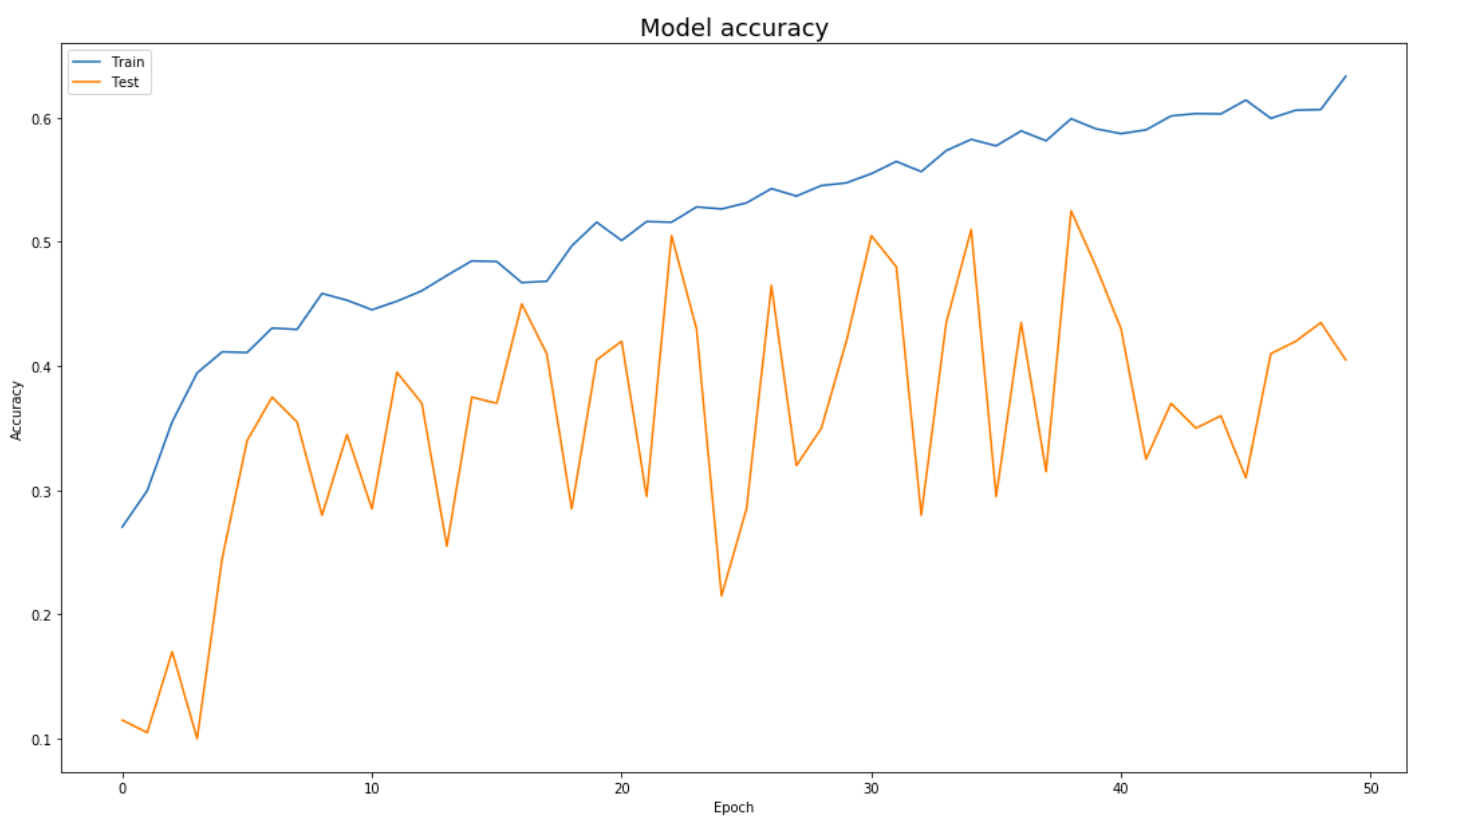
\includegraphics[width=0.85\textwidth]{model_acc}
	\center 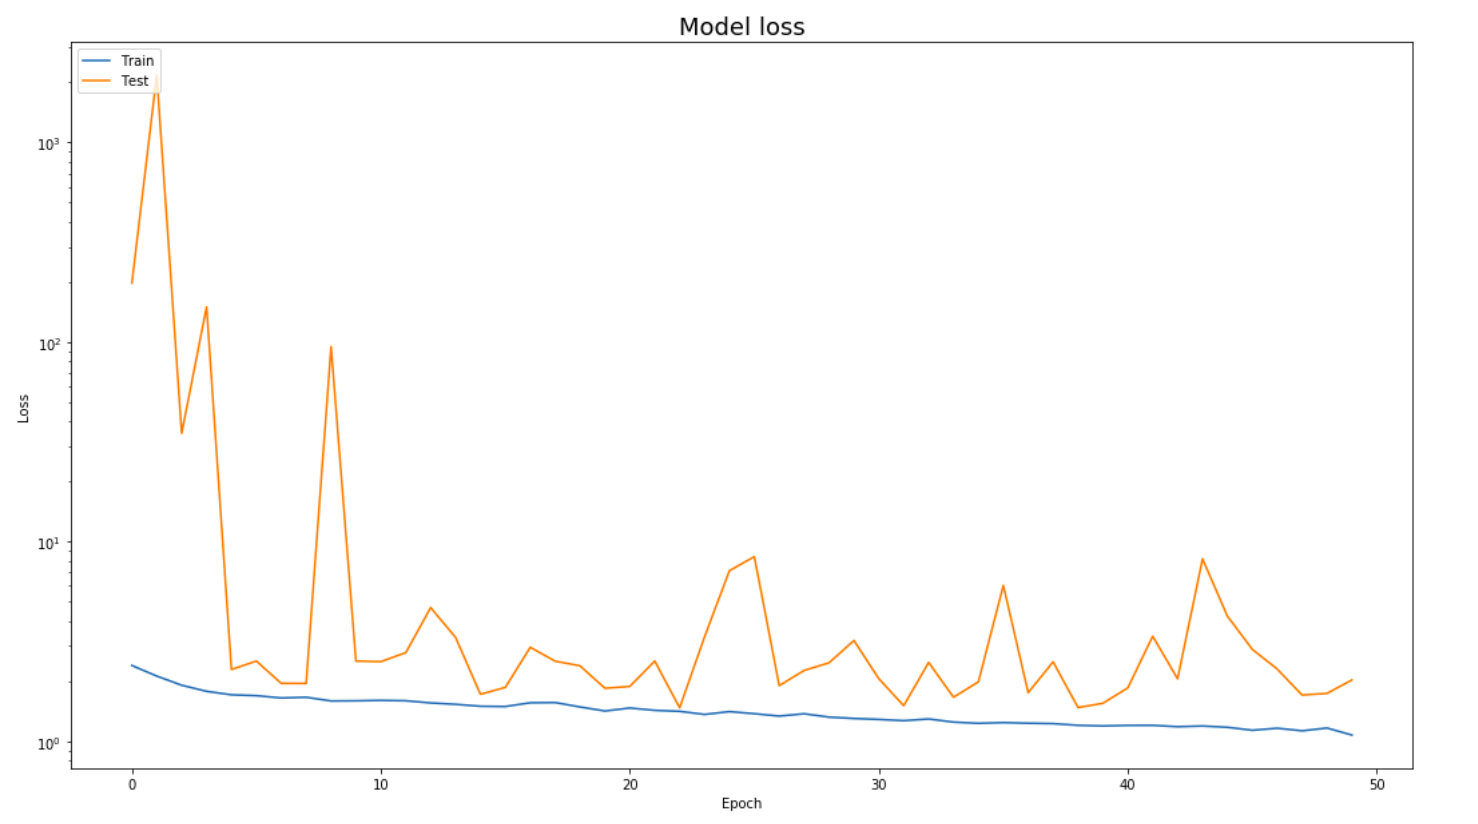
\includegraphics[width=0.85\textwidth]{model_loss}
	\caption{Training metrics: accuracy and loss for train and test datasets.}
\end{figure}

\pagebreak
In the same notebook, one can produce a prediction for a random image. Unfortunately, it also indicates that our model is severely overfitted.  As you can see the model returns the same prediction for each input image: it is always Renoir.\\

We have tried several different techniques to improve the predictions. We have tried a different amount of augmentation, tried to shuffle the images and split them again in train and test sets, we have also trained the whole model, all 50 layers on the training dataset (without transfer learning). All that did not bring us any significant improvement.\\

We assume that if this task even can be solved, it requires some specific model and a much larger dataset. Finding the difference in artists' styles seems to be far more difficult than an ordinary image recognition problem. 

\begin{figure}[H]
	\center 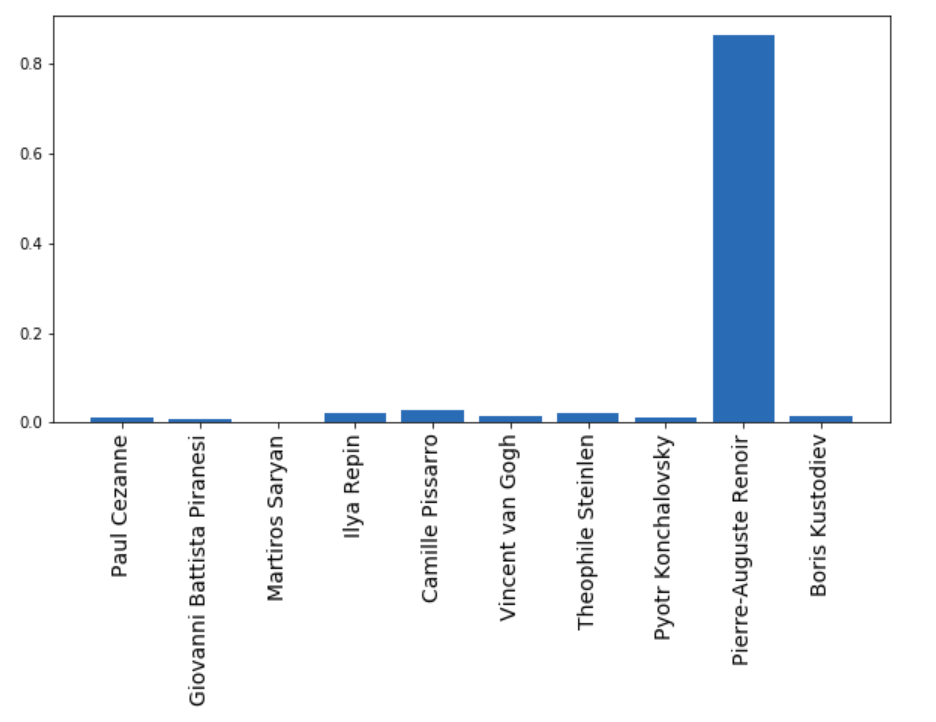
\includegraphics[width=0.85\textwidth]{prediction}
	\caption{Example prediction. The input image was in fact by \textit{Pyotr Konchalovsky}}
\end{figure}

 
\pagebreak
\section{Conclusion}

Further, we list some conclusions that we have made finishing this project.

\begin{enumerate}
	\item Keras simplifies the work with models but it has several restrictions, those are significant for using it on KF: 
	\begin{itemize}
		\item it cannot work directly with GCS buckets;
		\item it does not directly support distributed learning.
	\end{itemize}
	 \item Tensorflow is a very powerful tool but it requires additional learning time if you are not used to it. Another problem of Tensorflow is its rapid development, new versions of the framework have new interfaces for old functions, the structure of libraries changes significantly, which for example makes old tutorials useless. And Keras inside of Tensorflow and the stand-alone module can have different functions and structure although having the same version number.
	 \item Google Cloud Platform allows the dynamic managing of resources and has lots of other advantages. But the deployment of the Kunernetes cluster there has high costs. Previously we thought that the most expensive part will be training (on several CPUs or GPUs), but after all a simple maintaining of the "inactive" cluster takes most of the money. Luckily, the credits were provided for us and the whole project costs about \$60.
	 \item Kubeflow is still very raw. The actual version during the project was 0.5.0, it was still on the alpha stage. As an example, we can again refer to the replacing of \verb|ksonnet| through \verb|kustomize| without a large update of the documentation.\\
	 Another big disadvantage of Kubeflow from our perspective is that the user has to learn all underlying technologies like Kubernetes, Docker, \verb|kustomize|, etc.\\
	 Summarizing all this we suppose that Kubeflow does not suit for the research in data science: learning and maintaining it takes to many time and money if the tasks and technologies in your work often change. It is more reasonable to apply Kubeflow in production if the number of models is large but they do not differ a lot, if the models need to be constantly updated, or if the size of the data or the time constraints require distributed learning.
 \end{enumerate}

\pagebreak
\section{Acknowledgments}

We want to thank Google and Frankfurt Big Data Lab for providing free credits on GCP for this project, and also Todor Ivanov and Timo Eichhorn for the constant support.
\ \\
% Literaturverzeichnis
%\cleardoublepage
%\phantomsection
\addcontentsline{toc}{chapter}{Literaturverzeichnis}
\bibliography{literatur}

\begin{thebibliography}{7}

\bibitem{kf}
https://www.kubeflow.org/docs/

\bibitem{kaggle} 
https://www.kaggle.com/c/painter-by-numbers/

\bibitem{resnet} 
Kaiming He, Xiangyu Zhang, Shaoqing Ren, Jian Sun. \textit{Deep Residual Learning for Image Recognition}, arXiv:1512.03385

\bibitem{tf} 
https://www.tensorflow.org/guide

\bibitem{keras} 
https://keras.io/

\bibitem{kf_examples}
https://github.com/kubeflow/examples

\bibitem{kf_on_gcp}
https://www.kubeflow.org/docs/started/getting-started-gke/

\bibitem{k8s}
https://kubernetes.io/docs/concepts/workloads/pods/pod-overview/

\bibitem{gke}
https://cloud.google.com/kubernetes-engine/docs/how-to/gpus







 
\end{thebibliography}

\pagebreak
\section{Appendix}

\subsection*{Appendix 1. Commands used in the project}
\ \\
\begin{lstlisting}
# Specify environment variables
export PROJECT=painters-mnist
export DEPLOYMENT_NAME=kubeflow
export ZONE=us-central1-c
export VERSION_TAG=$(date +%s)
cd ~/git/painter-by-numbers
WORKING_DIR=$(pwd)

# Configure the GCP project
gcloud config set project ${PROJECT}
gcloud config set compute/zone ${ZONE}
gcloud auth login
gcloud container clusters get-credentials \
	${DEPLOYMENT_NAME} --zone ${ZONE} --project ${PROJECT}

# Set up kubectl
kubectl config set-context $(kubectl config current-context)\
	--namespace=kubeflow
kubectl get all

# Create GCS bucket
export BUCKET_NAME=${PROJECT}-${VERSION_TAG}
gsutil mb -c regional -l us-central1 gs://${BUCKET_NAME}

# Build, run(test localy) and push Docker image
export TRAIN_IMG_PATH=gcr.io/${PROJECT}/${DEPLOYMENT_NAME}-train-gpu:${VERSION_TAG}
sudo docker build $WORKING_DIR -t $TRAIN_IMG_PATH \
	-f $WORKING_DIR/Dockerfile_gpu.model
sudo docker run -it ${TRAIN_IMG_PATH}
gcloud auth configure-docker --quiet
sudo docker push ${TRAIN_IMG_PATH}

# Create a training pod
cd ${WORKING_DIR}/tfjobs
kubectl apply -f tfjob-gpu-args.yaml
\end{lstlisting}

\end{document}
